\chapter{Výsledky výzkumu a~diskuse}\label{vysledky}
Tato kapitola prezentuje výsledky provedeného experimentálního vyhodnocení a~následně je interpretuje z~hlediska praktické použitelnosti jednotlivých databázových systémů. 

Nejprve je popsán způsob zpracování a~agregace naměřených hodnot, poté jsou diskutovány výsledky výkonnostních testů, licenční omezení a~možnosti škálování jednotlivých řešení.

\section{Metodika Vyhodnocení}
Pro vyhodnocení byla použita pouze měření z~prostředí \texttt{remote}, tedy ze serveru poskytnutého DCÚK~(viz \ref{tab:hardwarespecs}). 

Pro testy \texttt{insert}, \texttt{single\_point}, \texttt{aggregate} a~\texttt{condition}
byl jako reprezentativní hodnota pro každou dvojici (databázový systém, profil) zvolen medián naměřené doby trvání dotazu namísto aritmetického průměru. 
Testovací kontejner totiž neběžel na fyzickém serveru jediný, ale běžel společně s~dalšími kontejnery, jejichž aktuální aktivita mohla dočasně způsobit výrazné zvýšení latence některých měření. 
Aritmetický průměr by byl na takové odlehlé hodnoty citlivý a~mohl by výsledky zkreslit, zatímco medián jejich vliv částečně potlačuje a~poskytuje stabilnější reprezentativní hodnotu.

Pro test typu \texttt{live\_insert} bylo vyhodnocení dále rozděleno podle kombinací testových parametrů \texttt{workers}~(2, 5 a 10) a~\texttt{batch\_size}~(1\,000, 10\,000 a 50\,000). Zatímco u~ostatních testů byly výsledky agregovány na úrovni jednotlivých profilů, v~tomto případě byla každá kombinace těchto parametrů posuzována samostatně.

Testy \texttt{insert} byly opakovány 33$\times$, testy \texttt{single\_point}, \texttt{aggregate} a~\texttt{condition} 100$\times$. Test \texttt{live\_insert} byl pro každou konfiguraci opakován 5$\times$. 

Již během pilotního testování byla zjištěna velmi nízká variabilita naměřených hodnot, a~proto nebylo nutné provádět rozsáhlejší počet opakování. Počet opakování byl tedy stanoven s~ohledem na kompromis mezi dostatečnou statisticky vypovídací hodnotou výsledků a~časovou náročností testování.

\section{Složitost instalace a konfigurace}
\label{sec:install-complexity}

Jako objektivní metrika instalační a~konfigurační náročnosti byl zvolen počet Ansible úloh potřebných k~plně automatizované instalaci a~konfiguraci daného systému v~rámci příslušné role (viz kapitola~\ref{sec:rolecommon}). 
Vzhledem k~tomu, že všechny role sdílejí stejnou strukturu (\texttt{tasks/install.yml}, případně \texttt{tasks/configure\_vm.yml} a~\texttt{tasks/setup\_database.yml}) a~stejnou úroveň rozdělení jednotlivých kroků, je počet úloh napříč systémy vzájemně srovnatelný a~odráží reálnou míru manuální práce, kterou by správce musel vykonat bez automatizace.

Hodnocení bylo, normalizováno na škálu 1--100 bodů, kde nejjednodušší systém (nejméně úloh) 
získává 100 bodů a~nejsložitější 1 bod.

\rowcolors{2}{gray!8}{white}
\begin{table}[H]
\centering
\caption{Instalační a~konfigurační náročnost databázových systémů}
\label{tab:install-complexity}

\begin{tabular}{l>{}cc@{}}
\toprule
\textbf{DBMS} & \textbf{Ansible úlohy} & \textbf{Normalizované skore} \\
\midrule
ClickHouse           & \best{9} & \best{100.00} \\
MongoDB              & 11 & 92.67\\
QuestDB              & 11 & 92.67\\
InfluxDB 3           & 13 & 85.33\\
MariaDB              & 22 & 52.33\\
MariaDB ColumnStore  & 22 & 52.33\\
TimescaleDB          & 28 & 30.33\\
Apache IoTDB         & \worst{36} & \worst{1.00} \\
\bottomrule
\end{tabular}
\end{table}
\rowcolors{2}{}{}

Z~tabulky~\ref{tab:install-complexity} vyplývá, že nejjednodušší instalaci ze všech testovaných systémů má \textbf{ClickHouse}, pouhých devět úloh zahrnujících přidání oficiálního APT repozitáře, import GPG klíče a~spuštění jediné služby \texttt{clickhouse-server}. 
Obdobně jednoduché jsou \textbf{MongoDB} a~\textbf{QuestDB}. MongoDB opět vystačí s~přidáním APT repozitáře, zatímco QuestDB je distribuováno jako samostatný binární 
archiv nevyžadující žádné systémové závislosti.

\textbf{InfluxDB~3} je instalačně také nenáročné, avšak na rozdíl od ostatních systémů vyžaduje ještě před prvním použitím vygenerování administrátorského API tokenu, bez 
kterého nelze do databáze zapisovat ani z~ní číst. 
Jedná se tak o~jediný testovaný systém, kde je autentizace vynucena už při~základním provozu, což mírně zvyšuje provozní (nikoliv čistě instalační) složitost.

\textbf{MariaDB} a~\textbf{MariaDB ColumnStore} vyžadují oproti výše zmíněným systémům citelně více kroků. Přidání vlastního repozitáře MariaDB, úpravu parametrů jádra (\texttt{sysctl}), vypnutí AppArmor a~nastavení kódování přijímaných dat. 
ColumnStore navíc potřebuje instalaci knihovny \texttt{jemalloc} a~konfiguraci tzv. CrossEngineSupport (vlastní databázový uživatel pro komunikaci mezi storage enginy InnoDB 
a~Columnstore).

\textbf{TimescaleDB} patří mezi náročnější systémy na konfiguraci. 
Instalace vyžaduje současné přidání dvou externích repozitářů (PostgreSQL PGDG a~TimescaleDB), následné doladění konfigurace nástrojem \texttt{timescaledb-tune} (příkaz sám upravuje nastavení TimescaleDB podle dostupných HW prostředků atd.), úpravu autentizační metody v~\texttt{pg\_hba.conf} (výchozí nastavení znemožňuje strojové připojení) a~explicitní vynucení načtení rozšíření přes \texttt{shared\_preload\_libraries}.

Nejsložitější instalaci a~konfiguraci ze všech testovaných systémů má jednoznačně \textbf{Apache IoTDB}, se 36 dílčími úlohami. 
Systém vyžaduje instalaci Java runtime (OpenJDK 17), ladění parametrů jádra, dočasné vypnutí a~zapnutí swapu, navýšení limitů otevřených souborů a~ruční výpočet velikosti Java heapu\footnote{\textit{Java Heap} - vyhrazené místo v paměti pro ukládání mezivýsledků v JVM (Java Virtual Machine)} (\texttt{MAX\_HEAP\_SIZE}) pro ConfigNode a~DataNode na základě přidělené paměti kontejneru.
Architektura navíc i~pro jednouzlové nasazení vyžaduje současný běh dvou nezávislých služeb (ConfigNode a~DataNode), které je nutné spouštět a~monitorovat odděleně.

\section{Výkonnost}\label{sec:performance}
Následující podkapitoly shrnují výsledky jednotlivých testů definovaných 
v~sekci \ref{sec:test_implementation}. U~testů \texttt{insert}, 
\texttt{single\_point}, \texttt{aggregate} a~\texttt{condition} je uváděn 
medián doby trvání dotazu měřený přímo na straně databázového serveru. 

U~testu \texttt{live\_insert} je uváděn medián propustnosti (vložených řádků za sekundu testu).

Hodnocení jednotlivých databází pro klasické testy je normalizováno na škálu 1--100 bodů: nejrychlejší systém v~daném testu získává 100 bodů, nejpomalejší 1 bod a~
ostatní jsou lineárně rozloženy mezi ně. 
Celkový výsledek je aritmetický průměr z~jednotlivých testů. 
Nejlepší databázový systém je ten s~nejvyšším počtem bodů a~tabulky jsou podle toho i~seřazeny. 
Test \texttt{live\_insert} není zahrnut do celkového hodnocení, 
jelikož jeho charakter vyžaduje odlišnou metodiku a~vizualizaci.

Testování probíhalo na třech hardwarových profilech s~postupně navyšujícím se 
množstvím přidělených prostředků (\texttt{small}, \texttt{medium} a~\texttt{large}, 
viz sekci~\ref{sec:implementacetestu}), aby bylo možné posoudit nejen absolutní 
výkon jednotlivých systémů, ale i~to, jak efektivně dokážou dodatečné výpočetní 
prostředky využít. Následující podkapitoly prezentují výsledky pro jednotlivé 
profily zvlášť, přičemž jejich vzájemné porovnání a~diskuse škálovatelnosti je 
uvedena v~sekci~\ref{sec:scaling}.
\clearpage
\subsection{Small (1 CPU Core, 2\,GiB RAM)}
Pro tento profil byla použita hardwarová konfigurace 1 jádro CPU a~2\,GiB RAM.

\rowcolors{2}{gray!8}{white}
\begin{table}[H]
\centering
\caption{Výsledky benchmarku na profilu \texttt{small}}
\label{tab:benchmark-small}

\begin{tabular}{@{}lcccc>{}c@{}}
\toprule
\textbf{DBMS} & \textbf{Insert} & \textbf{Single point} & \textbf{Condition} & \textbf{Aggregate} & \textbf{Průměr bodů} \\
\midrule

ClickHouse & \best{100.00} & 85.86 & \best{100.00} & \best{100.00} & \best{96.47} \\
TimescaleDB & 71.71 & 57.57 & 71.71 & 71.71 & 68.17 \\
InfluxDB 3 & 29.29 & \best{100.00} & 85.86 & 43.43 & 64.64 \\
QuestDB & 43.43 & 43.43 & 57.57 & 85.86 & 57.57 \\
MariaDB ColumnStore & 85.86 & 29.29 & 29.29 & 57.57 & 50.50 \\
Apache IoTDB & \worst{1.00} & 71.71 & 43.43 & 29.29 & 36.36 \\
MariaDB & 57.57 & 15.14 & 15.14 & 15.14 & 25.75 \\
MongoDB & 15.14 & \worst{1.00} & \worst{1.00} & \worst{1.00} & \worst{4.54} \\
\bottomrule
\end{tabular}
\end{table}
\rowcolors{2}{}{}

Z~tabulky~\ref{tab:benchmark-small} vyplývá, že nejlepším databázovým 
systémem pro klasické testy na tomto profilu je \textbf{ClickHouse}. 
Zajímavé je extrémní propadnutí MongoDB, které ve všech testech kromě 
\texttt{insert} dosáhlo nejhorších výsledků.

\begin{figure}[H]
    \centering
    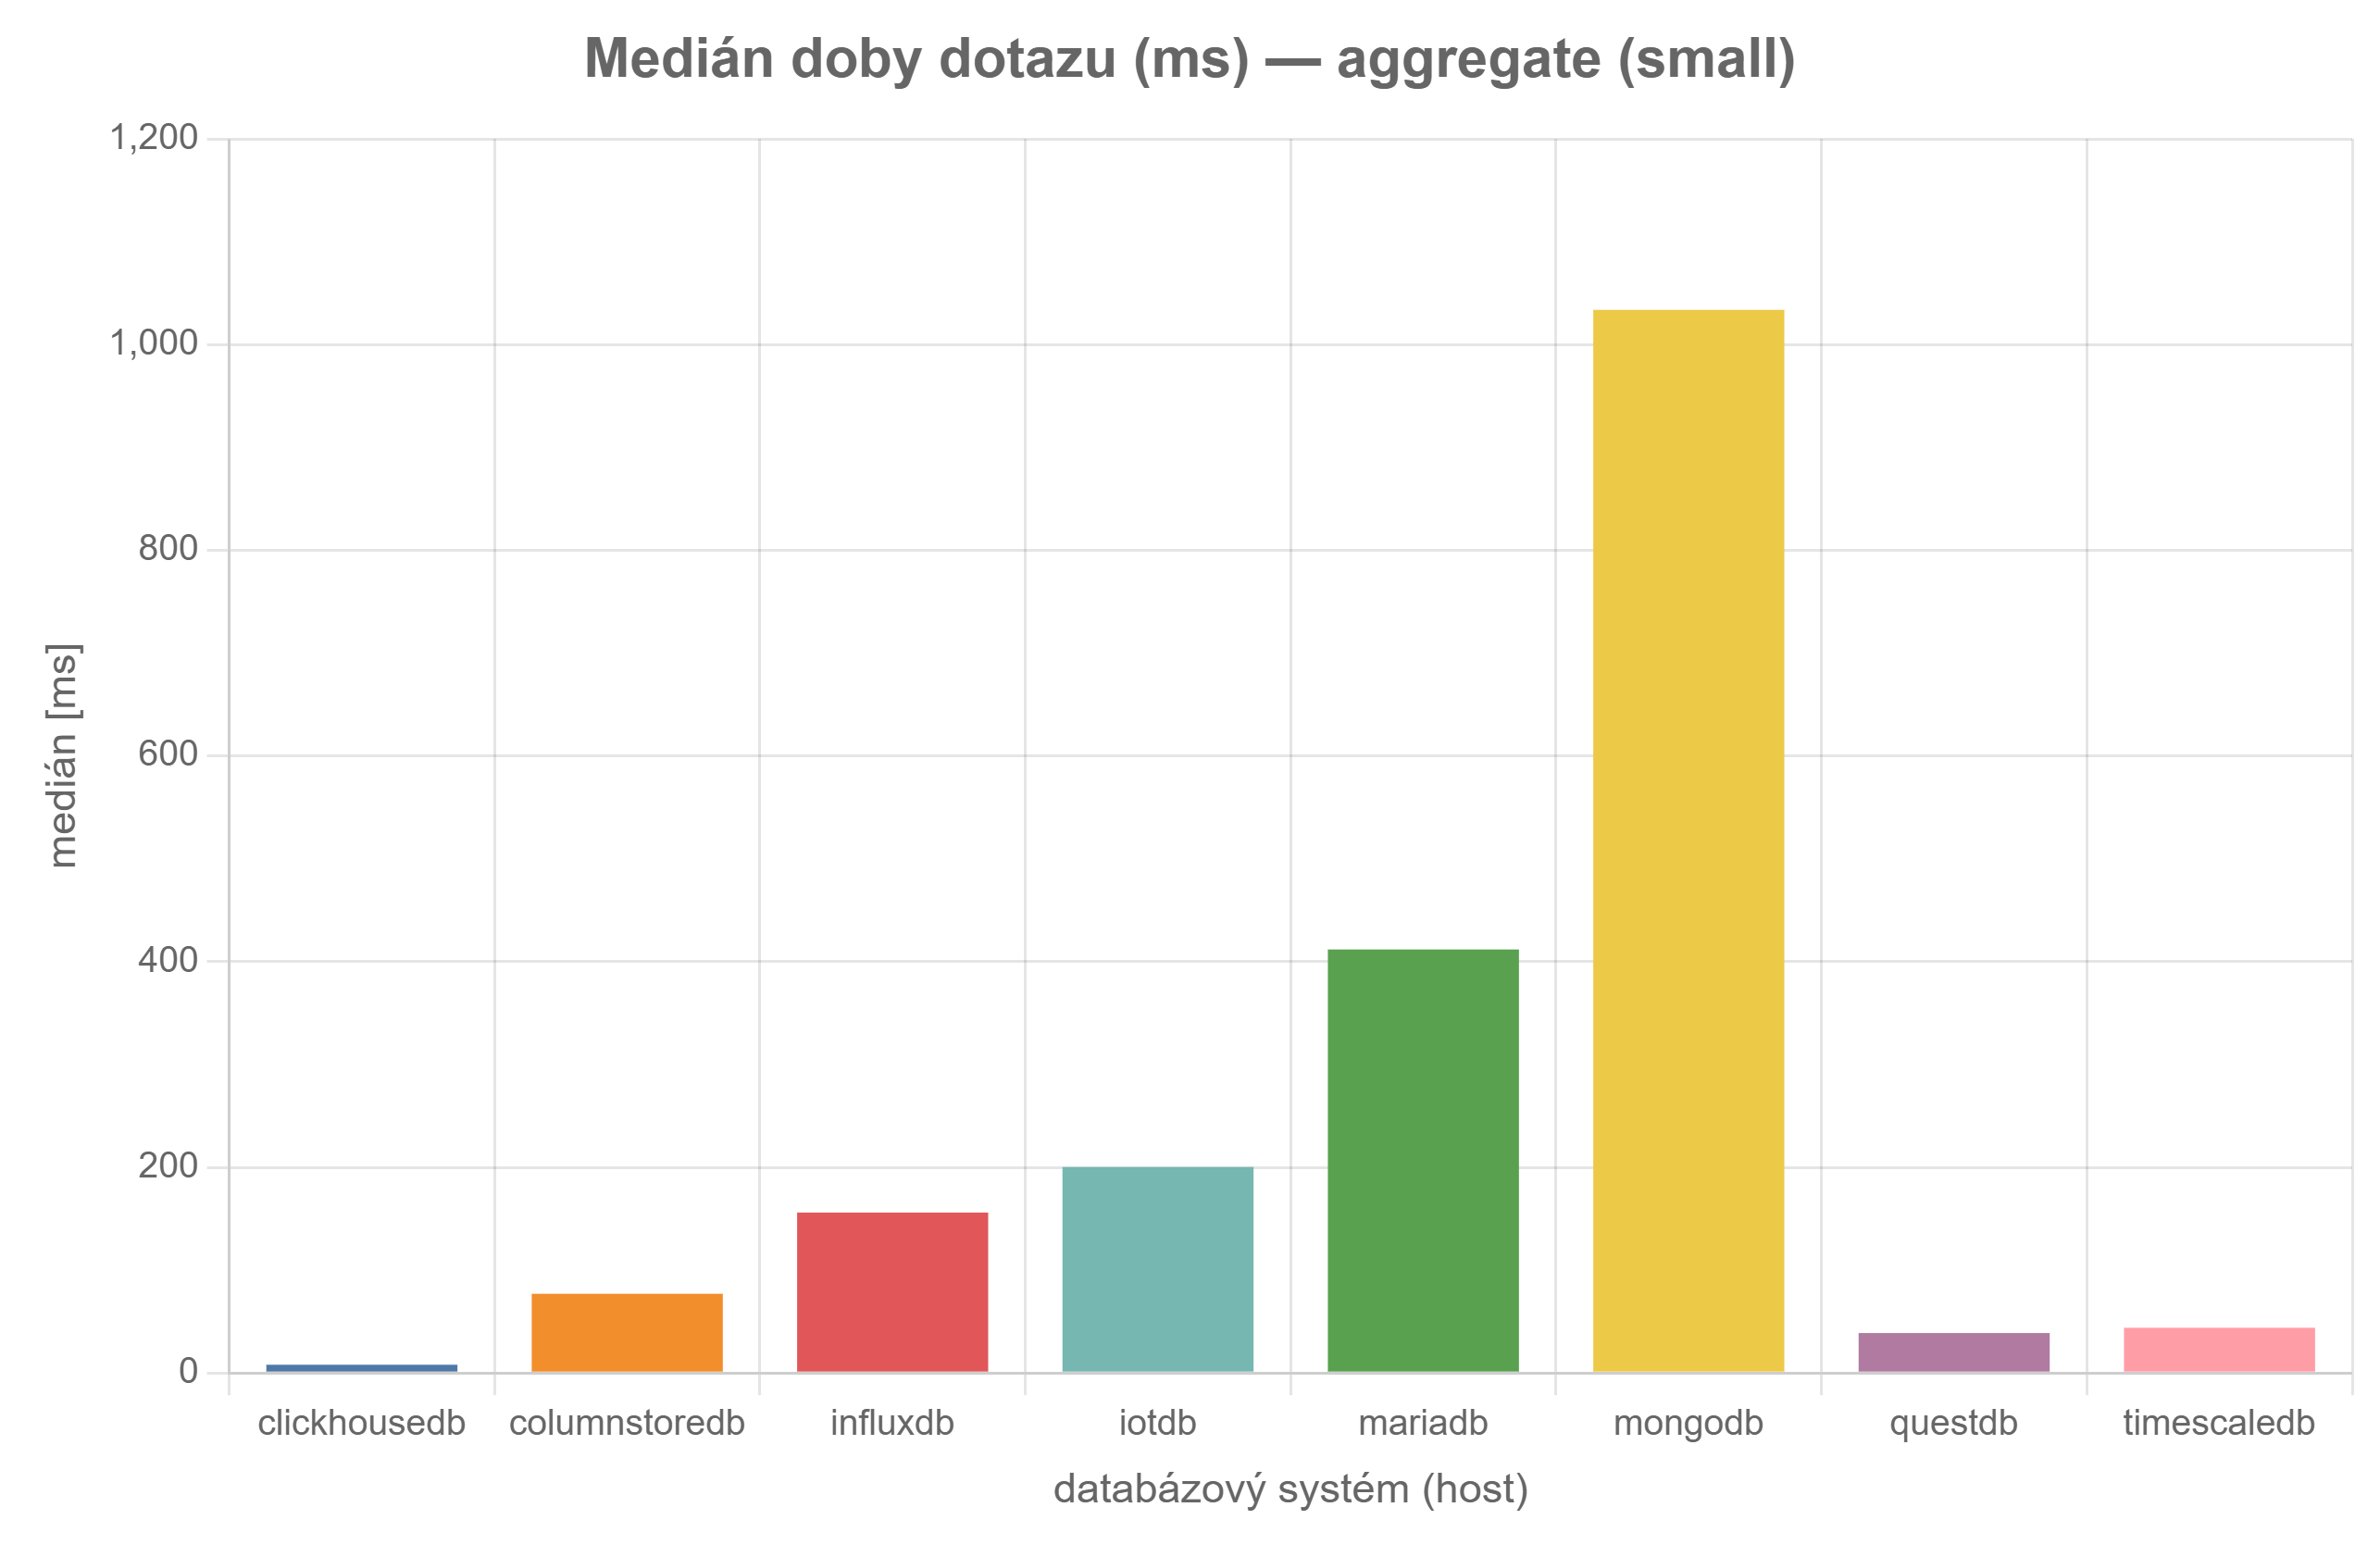
\includegraphics[width=0.7\textwidth]{images/small_aggregate.png}
    \caption{Medián doby trvání dotazu \texttt{aggregate} na profilu 
             \texttt{small} (zdroj: Vlastní zpracování)}
    \label{fig:small_aggregate}
\end{figure}

V~konkrétních číslech dosáhl medián doby trvání dotazu \texttt{aggregate} 
v~ClickHouse pouhých \textbf{8\,ms}, zatímco MongoDB potřeboval 
\textbf{1033\,ms} (tedy přibližně 130$\times$ déle).

Na obrázku~\ref{fig:mongodb_small_aggregate} je zachycen detailní průběh 
CPU a~paměti MongoDB na samotném začátku testu \texttt{aggregate}. 

\begin{figure}[H]
    \centering
    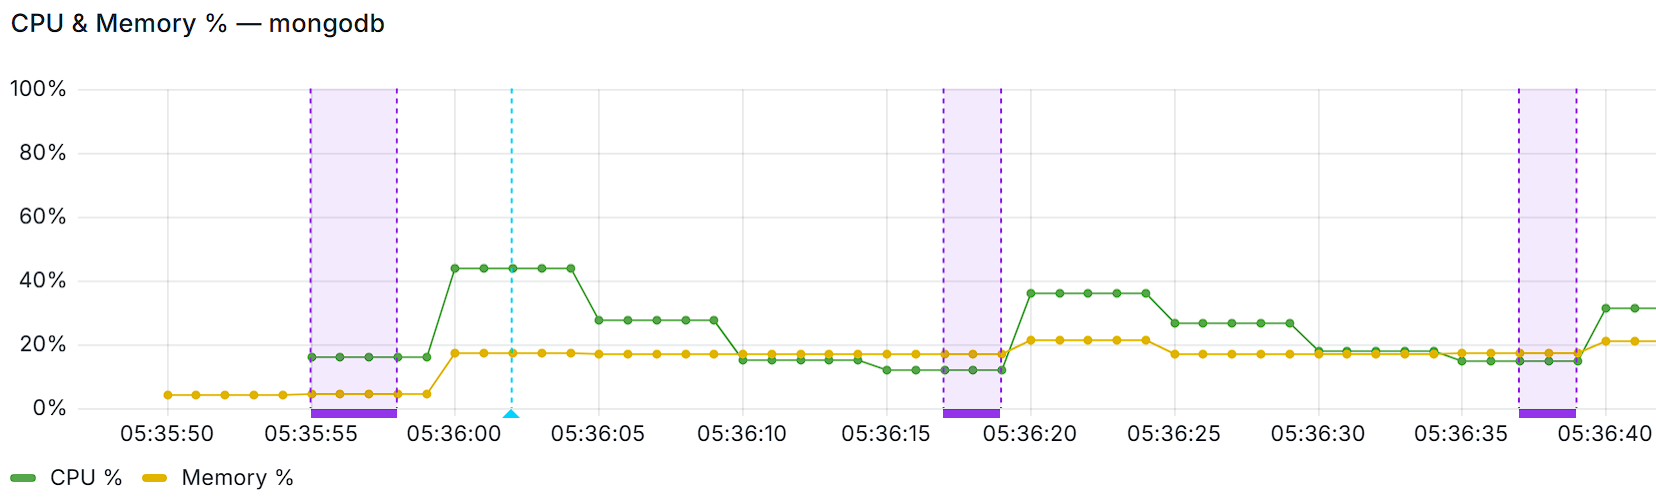
\includegraphics[width=0.9\textwidth]{images/mongodb_small_aggregate.png}
    \caption{Měření CPU a~RAM pro test \texttt{aggregate} u~MongoDB (zdroj: Vlastní zpracování)}
    \label{fig:mongodb_small_aggregate}
\end{figure}

Na samotném začátku \texttt{aggregate} testu u~MongoDB lze vidět, že 
paměť stoupne na 17,4\,\% (modré znázornění v~grafu \ref{fig:mongodb_small_aggregate}), což odpovídá více než 100\,MB paměti. Tím 
překročí výchozí limit pro jednotlivé stupně agregační pipeline a~
MongoDB musí část mezivýsledků zapsat na disk, což několikanásobně zpomalí trvání dotazu. \cite{mongodbaggregate}. 

Současně lze pozorovat, že CPU (zelená křivka) se v~těchto fázích drží 
na 40--45\,\%, tedy procesor není plně využíván. To potvrzuje, že 
limitujícím faktorem není výpočetní výkon, ale právě diskový I/O~způsobený 
výše zmíněným chováním.

\subsubsection{Live insert}
Následující tabulka prezentuje naměřenou propustnost při kontinuálním vkládání dat v reálném čase.

\rowcolors{2}{gray!8}{white}
\begin{table}[H]
\centering
\caption{Propustnost \texttt{live\_insert} (řádky/s) na profilu \texttt{small}}
\label{tab:live-insert-small}
\resizebox{\textwidth}{!}{%
\begin{tabular}{@{}lccccccccc>{}c@{}}
\toprule
\textbf{DBMS} & \textbf{2/1k} & \textbf{5/1k} & \textbf{10/1k} & \textbf{2/10k} & \textbf{5/10k} & \textbf{10/10k} & \textbf{2/50k} & \textbf{5/50k} & \textbf{10/50k} & \textbf{Průměrná propustnost} \\
\midrule
ClickHouse & 9634 & 9984 & \best{11225} & \best{14022} & \best{14034} & \best{13302} & \best{13887} & \best{13152} & \best{10517} & \best{\textbf{12195}} \\
TimescaleDB & \best{11177} & \best{10969} & 10802 & 11452 & 11644 & 11472 & 11442 & 11785 & 9741 & \textbf{11165} \\
MariaDB & 10016 & 9920 & 9764 & 9851 & 9993 & 9420 & 9765 & 9591 & \worst{--} & \textbf{8702} \\
MongoDB & 8409 & 8161 & 8033 & 9015 & 8684 & 8299 & 8571 & 8543 & 7550 & \textbf{8363} \\
Apache IoTDB & 6343 & 5843 & 5535 & 8854 & 8031 & 7936 & 9155 & 7896 & 5718 & \textbf{7257} \\
InfluxDB 3 & 6856 & 6816 & 6723 & 6891 & 6835 & 6897 & \worst{6757} & 6656 & 5591 & \textbf{6669} \\
QuestDB & 5925 & 5918 & 5847 & 7093 & 6548 & 5941 & 7310 & 5899 &  4423 & \textbf{6100} \\
MariaDB ColumnStore & \worst{1100} & \worst{1062} & \worst{1030} & \worst{3277} & \worst{3131} & \worst{2764} & 7415 & \worst{5744} & \worst{--} & \worst{\textbf{3190}} \\
\bottomrule
\end{tabular}}
\end{table}
\rowcolors{2}{}{}

Z~tabulky~\ref{tab:live-insert-small} vyplývá, že ClickHouse dosahuje nejvyšší průměrné propustnosti (12\,195 řádků/s) a~dominantní pozice při~větších dávkách (10\,000 a~50\,000 řádků). 
To odpovídá jeho architektuře optimalizované pro batchové zpracování velkých objemů dat.

Zároveň je patrné, že u~všech sledovaných databázových systémů dochází při~kombinaci vysoké paralelizace a~velké velikosti dávky ke snížení dosažené propustnosti. Při~omezeném počtu dostupných procesorových jader může příliš vysoká míra paralelizace vést k~nárůstu režie spojené s~řízením vláken a~přepínáním kontextu, což může negativně ovlivnit výsledný výkon.

Při~malých dávkách (1\,000 řádků), které simulují typický IoT scénář, časté zápisy malých souborů z~mnoha zařízení, překonává ClickHouse \mbox{TimescaleDB}, který dosahuje 
nejvyšší propustnosti pro konfigurace 2/1k a~5/1k (11\,177, resp. 10\,969 řádku/s).

Pro konfiguraci 10/50k nejsou u~MariaDB a~u~MariaDB ColumnStore uvedena data, neboť při~tomto nastavení již databázový systém nedokáže v~rámci časového limitu zpracovat vkládaná data.

\subsection{Medium (2 CPU Core, 4\,GiB RAM)}
Pro tento profil byla použita hardwarová konfigurace 2 jádra CPU a~4\,GiB RAM.

\rowcolors{2}{gray!8}{white}
\begin{table}[H]
\centering
\caption{Výsledky benchmarku na profilu \texttt{medium}}
\label{tab:benchmark-medium}

\begin{tabular}{@{}lcccc>{}c@{}}
\toprule
\textbf{DBMS} & \textbf{Insert} & \textbf{Single point} & \textbf{Condition} & \textbf{Aggregate} & \textbf{Průměr bodů} \\
\midrule
ClickHouse & \best{100.00} & 85.86 & \best{100.00} & \best{100.00} & \best{\textbf{96.47}} \\
TimescaleDB & 71.71 & 43.43 & 71.71 & 71.71 & \textbf{64.64} \\
InfluxDB 3 & 29.29 & \best{100.00} & 85.86 & 43.43 & \textbf{64.64} \\
QuestDB & 43.43 & 57.57 & 43.43 & 85.86 & \textbf{57.57} \\
MariaDB ColumnStore & 85.86 & 29.29 & 29.29 & 57.57 & \textbf{50.50} \\
Apache IoTDB & \worst{1.00} & 71.71 & 57.57 & 29.29 & \textbf{39.89} \\
MariaDB & 57.57 & 15.14 & 15.14 & 15.14 & \textbf{25.75} \\
MongoDB & 15.14 & \worst{1.00} & \worst{1.00} & \worst{1.00} & \worst{\textbf{4.54}} \\
\bottomrule
\end{tabular}
\end{table}
\rowcolors{2}{}{}

Z~tabulky~\ref{tab:benchmark-medium} vyplývá, že nejlepším databázovým systémem pro klasické testy i~na tomto profilu zůstává \textbf{ClickHouse}. 

\textbf{Apache IoTDB} má zdaleka nejpomalejší \texttt{insert}, kde dosáhl výrazně nejhoršího výsledku ze všech systémů. 
Je 3$\times$ pomalejší než druhý nejhorší systém v~tomto typu testu, MongoDB.

\begin{figure}[H]
    \centering
    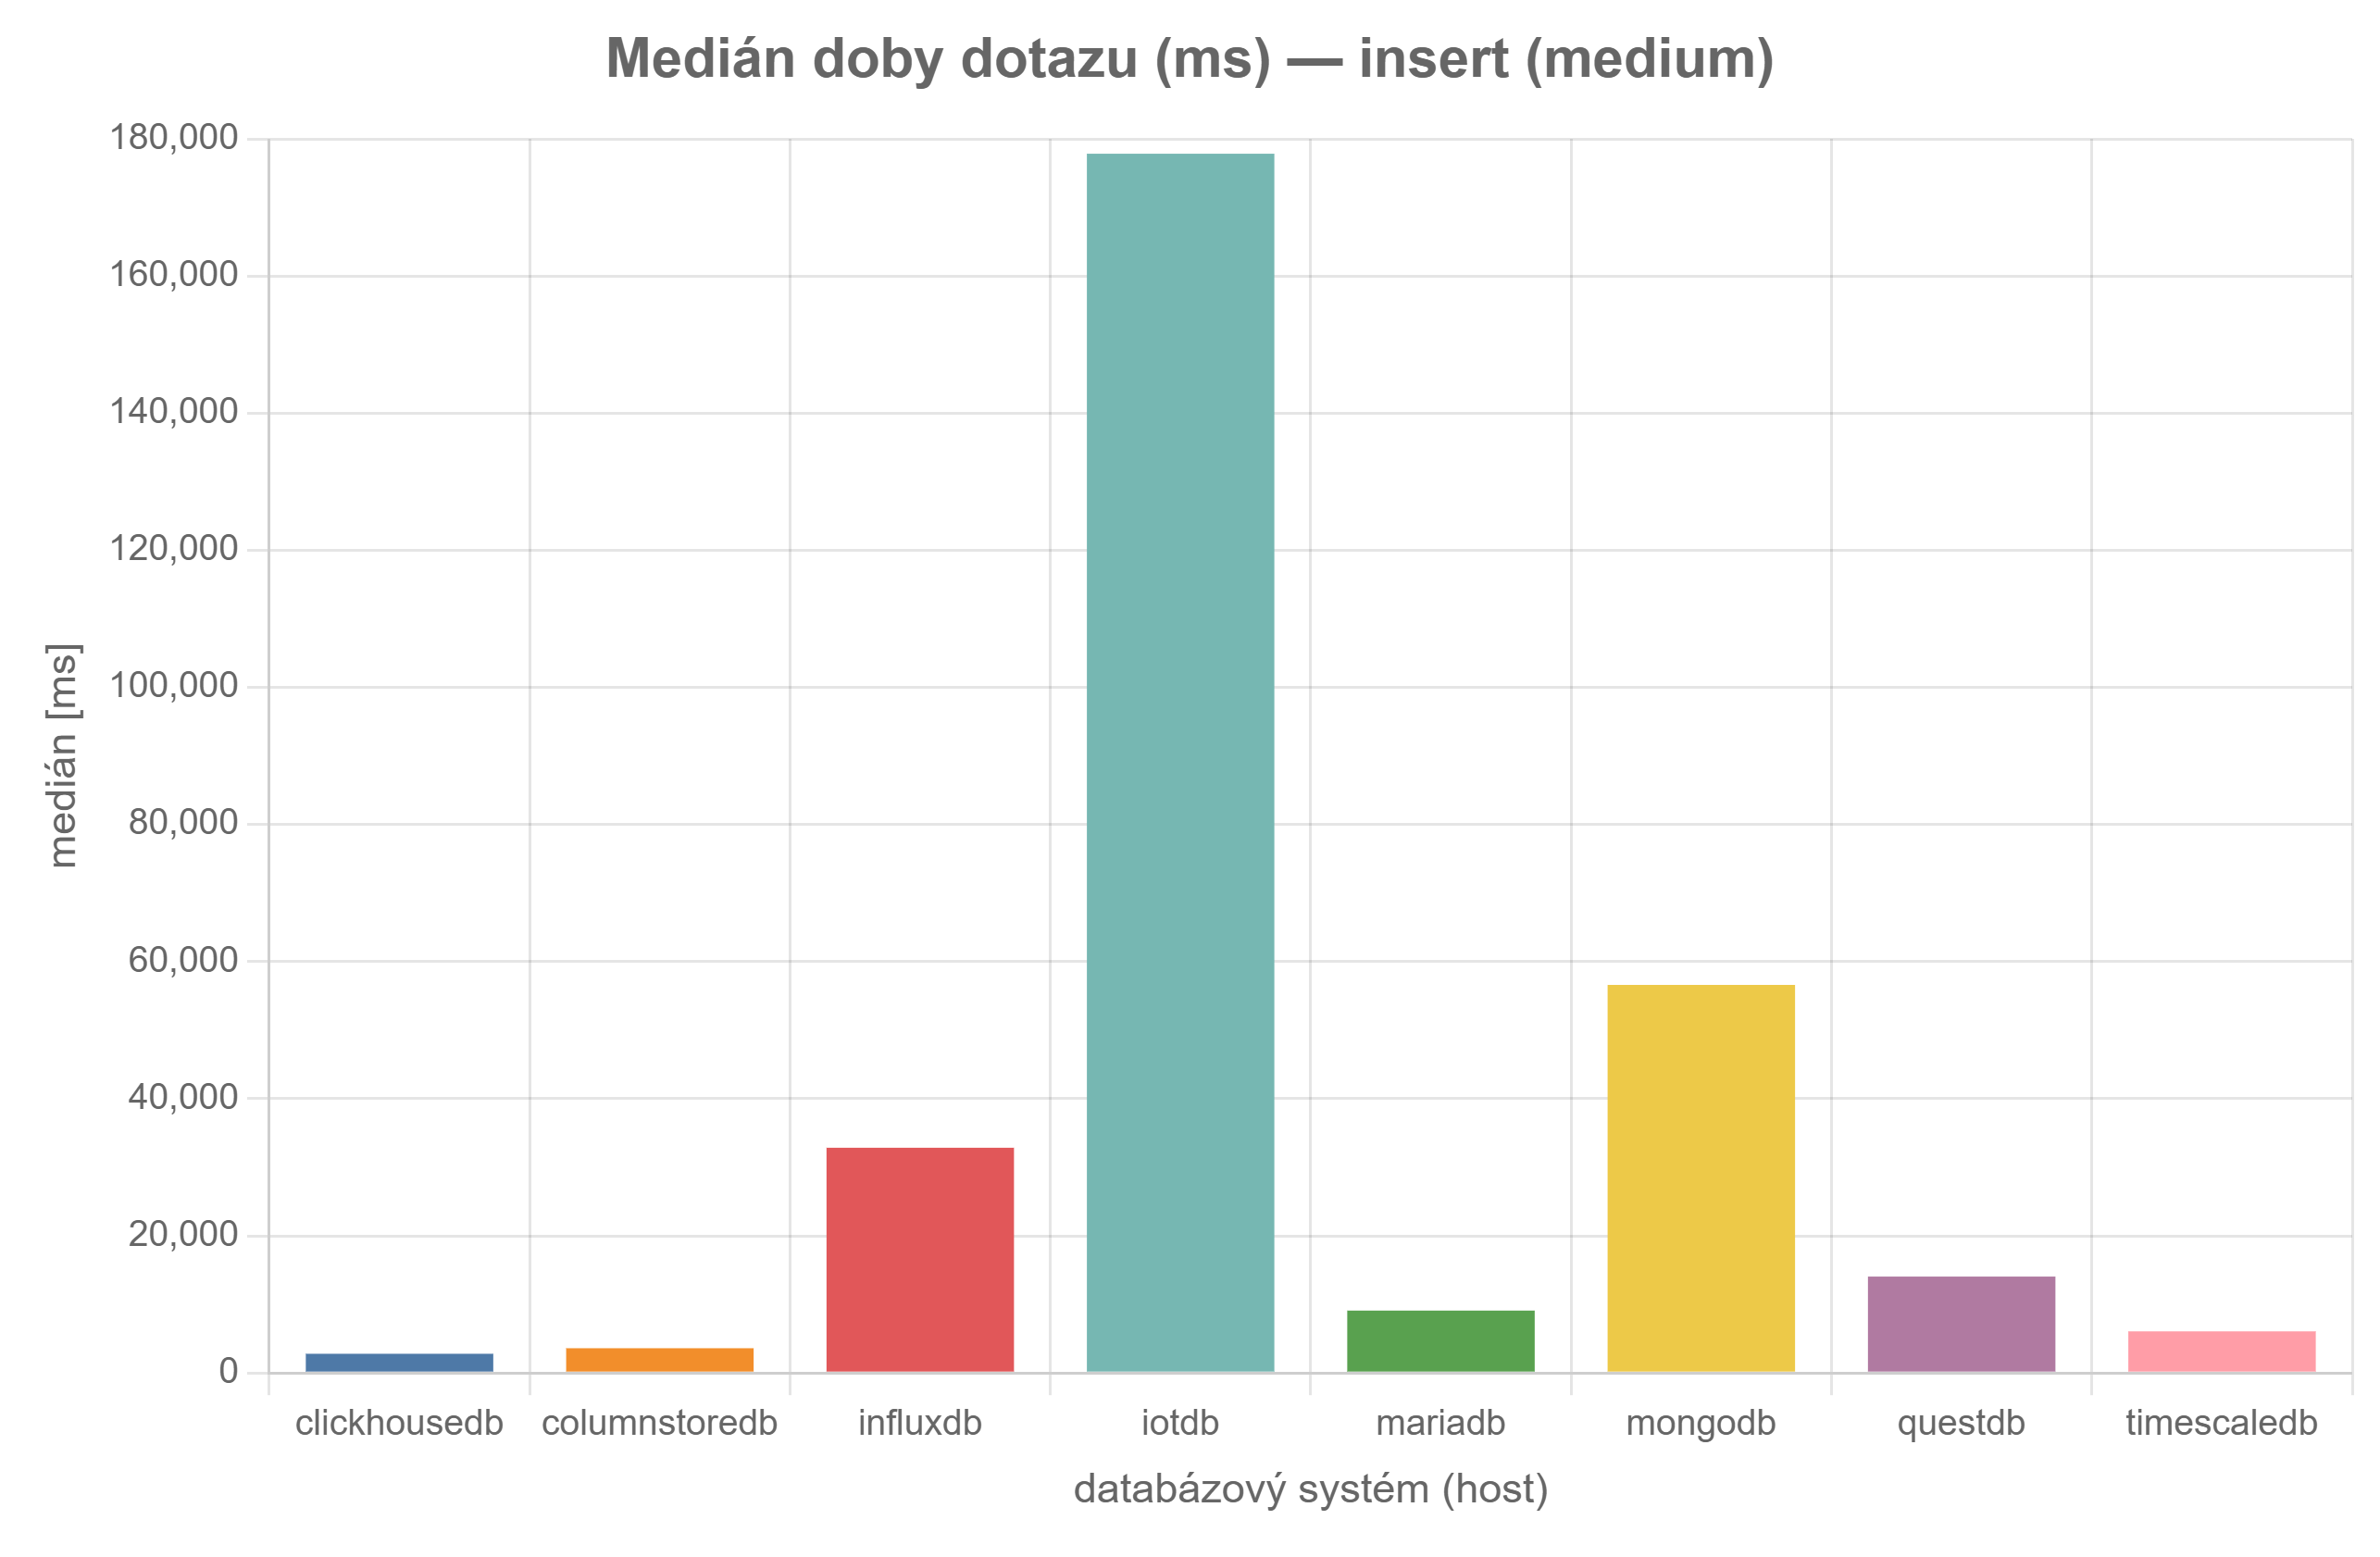
\includegraphics[width=0.9\textwidth]{images/medium_insert.png}
    \caption{Medián doby trvání dotazu \texttt{insert} na profilu 
             \texttt{medium} (zdroj: Vlastní zpracování)}
    \label{fig:medium_insert}
\end{figure}

V~konkrétních číslech dosáhl medián doby trvání dotazu \texttt{insert} v~ClickHouse pouhých \textbf{2\,800\,ms}, zatímco Apache IoTDB potřebovalo \textbf{177\,000\,ms} (tedy přibližně 63,5$\times$ déle). 

Toto chování odpovídá architektuře IoTDB, která je primárně navržena 
pro edge/IoT scénáře s~distribuovanými zápisy z~mnoha malých zařízení, 
nikoliv pro masivní synchronní bulk insert na jediném serveru s~
omezenými zdroji.

Na grafu \ref{fig:iotdb-medium-cpu} je zachycen průběh CPU a~paměti Apache IoTDB během testu \texttt{insert}. 
Zelená křivka reprezentuje vytížení procesoru, žlutá využití operační paměti.

\begin{figure}[H]
    \centering
    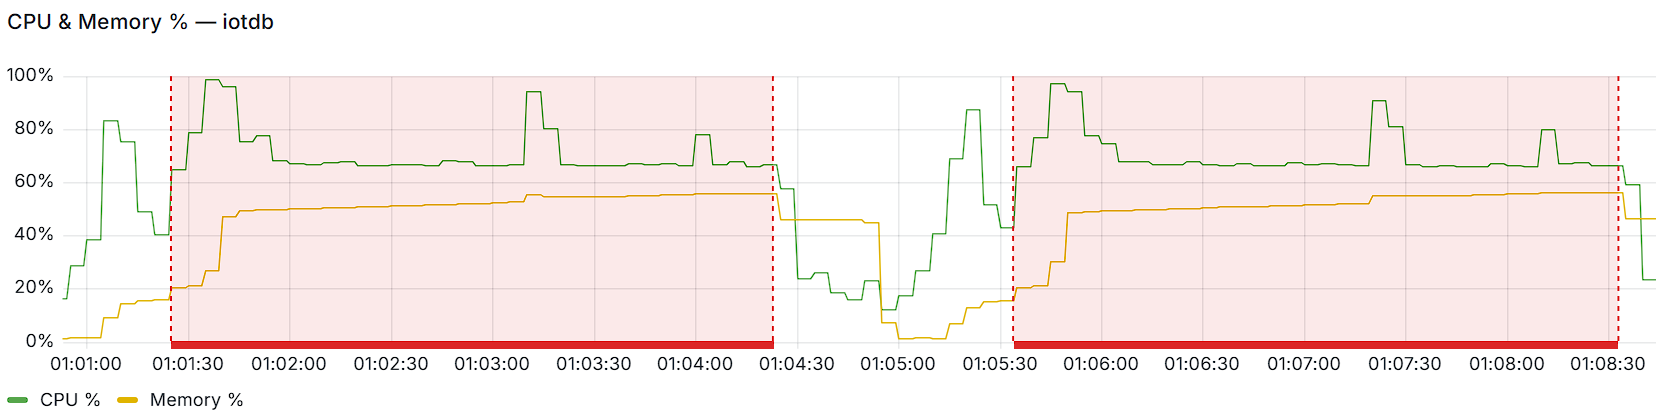
\includegraphics[width=1\textwidth]{images/iotdb-medium-cpu.png}
    \caption{Vytížení CPU a~paměti Apache IoTDB během testu 
             \texttt{insert} na profilu \texttt{medium} (zdroj: Vlastní zpracování)}
    \label{fig:iotdb-medium-cpu}
\end{figure}

Z~grafu je patrné, že CPU se po celou dobu insertu drží na 80--100\,\%, zatímco paměť postupně roste až na přibližně 60\,\% celkové kapacity. 
To naznačuje, že IoTDB je při~tomto testu výrazně limitováno výkonem procesoru.

\begin{figure}[H]
    \centering
    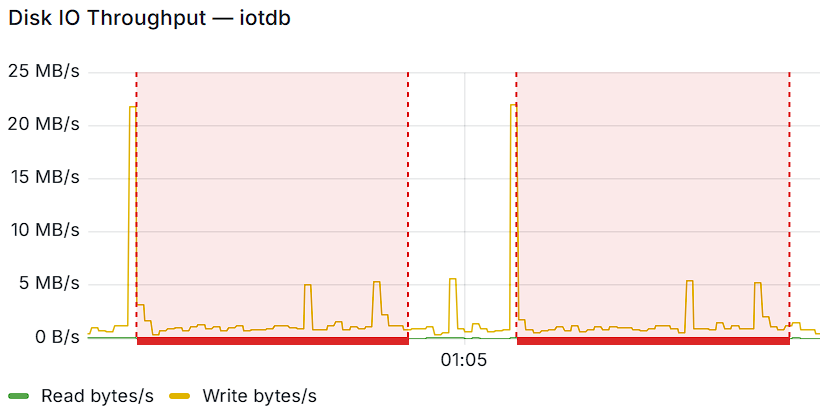
\includegraphics[width=1\textwidth]{images/iotdb-medium-disk.png}
    \caption{Diskový I/O~Apache IoTDB během testu \texttt{insert} na profilu \texttt{medium}.}
    \label{fig:iotdb-medium-disk}
\end{figure}

Graf \ref{fig:iotdb-medium-disk} potvrzuje, že diskový I/O~vykazuje pouze krátké špičky zápisů, nikoliv kontinuální vytížení. Limitujícím faktorem tedy není propustnost úložiště, ale právě vnitřní zpracování dat v~paměti a~výkon procesru.

\subsubsection{Live insert}
Pro střední hardwarový profil byl test živého zápisu opětovně proveden s různými kombinacemi počtu workerů a velikosti dávky.

\rowcolors{2}{gray!8}{white}
\begin{table}[H]
\centering
\caption{Propustnost \texttt{live\_insert} (řádky/s) na profilu \texttt{medium}}
\label{tab:live-insert-medium}
\resizebox{\textwidth}{!}{%
\begin{tabular}{@{}lccccccccc>{}c@{}}
\toprule
\textbf{DBMS} & \textbf{2/1k} & \textbf{5/1k} & \textbf{10/1k} & \textbf{2/10k} & \textbf{5/10k} & \textbf{10/10k} & \textbf{2/50k} & \textbf{5/50k} & \textbf{10/50k} & \textbf{Průměrná propustnost} \\
\midrule
ClickHouse & 14818 & 16071 & 21195 & \best{25942} & \best{27062} & \best{27492} & \best{27951} & \best{27018} & \best{26939} & \best{\textbf{23832}} \\
TimescaleDB & \best{21975} & \best{22385} & \best{22071} & 22301 & 23514 & 22413 & 23794 & 22473 & 22769 & \textbf{22633} \\
MariaDB & 18086 & 18695 & 18783 & 19303 & 19493 & 19053 & 18434 & 17917 & 17547 & \textbf{18590} \\
MongoDB & 16187 & 15809 & 15596 & 17284 & 16972 & 16627 & 16888 & 16569 & 16362 & \textbf{16477} \\
Apache IoTDB & 13513 & 12267 & 11785 & 18031 & 17280 & 16084 & 18164 & 17770 & 15494 & \textbf{15599} \\
QuestDB & 11706 & 11972 & 11770 & 14805 & 14666 & 14158 & 16285 & 15450 & 14577 & \textbf{13932} \\
InfluxDB 3 & 13066 & 12899 & 13070 & 13243 & 12942 & 13090 & 12852 & 12493 & 12828 & \textbf{12943} \\
MariaDB ColumnStore & \worst{1210} & \worst{1288} & \worst{1174} & \worst{3613} & \worst{3588} & \worst{3423} & \worst{10435} & \worst{9414} & \worst{8163} & \worst{\textbf{4701}} \\
\bottomrule
\end{tabular}}
\end{table}
\rowcolors{2}{}{}

Z tabulky \ref{tab:live-insert-medium} vyplývá, že ClickHouse znovu dosahuje nejvyšší průměrné propustnosti, a~to \mbox{23,832 řádků/s}.
Na tomto profilu se však TimescaleDB výrazně přiblížil (22\,633 řádků/s) a při konfiguraci \texttt{10/1k} dokonce překonal ClickHouse. 

Apache IoTDB se v~live insert chová výrazně lépe než v~klasickém synchronním insertu, což potvrzuje, že jeho architektura lépe vyhovuje asynchronnímu nahrávání menších dávek.

MariaDB i~MariaDB ColumnStore jsou již schopné na aktuální hardwarové konfigurace všechny testy dokončit.

\subsection{Large (4 CPU Core, 8\,GiB RAM)}
Pro tento profil byla použita hardwarová konfigurace 4 jádra CPU a~8\,GiB RAM.

\rowcolors{2}{gray!8}{white}
\begin{table}[H]
\centering
\caption{Výsledky benchmarku na profilu \texttt{large}}
\label{tab:benchmark-large}

\begin{tabular}{@{}lcccc>{}c@{}}
\toprule
\textbf{DBMS} & \textbf{Insert} & \textbf{Single point} & \textbf{Condition} & \textbf{Aggregate} & \textbf{Průměr bodů} \\
\midrule
ClickHouse & \best{100.00} & 85.86 & \best{100.00} & \best{100.00} & \best{\textbf{96.47}} \\
QuestDB & 43.43 & 57.57 & 57.57 & 85.86 & \textbf{61.11} \\
InfluxDB 3 & 29.29 & \best{100.00} & 85.86 & 29.29 & \textbf{61.11} \\
TimescaleDB & 71.71 & 43.43 & 43.43 & 71.71 & \textbf{57.57} \\
MariaDB ColumnStore & 85.86 & 29.29 & 29.29 & 57.57 & \textbf{50.50} \\
Apache IoTDB & \worst{1.00} & 71.71 & 71.71 & 43.43 & \textbf{46.96} \\
MariaDB & 57.57 & 15.14 & 15.14 & 15.14 & \textbf{25.75} \\
MongoDB & 15.14 & \worst{1.00} & \worst{1.00} & \worst{1.00} & \worst{\textbf{4.54}} \\
\bottomrule
\end{tabular}
\end{table}
\rowcolors{2}{}{}

Z~tabulky~\ref{tab:benchmark-large} vyplývá, že nejlepším databázovým systémem pro klasické testy i~na tomto profilu zůstává \textbf{ClickHouse}.
Opakuje se tak stejný vzor jako u~profilů \texttt{small} a~\texttt{medium}, kdy ClickHouse suverénně vede ve třech ze čtyř testů a~celkově dosahuje skóre 96,47 bodu. 

Při~přechodu na větší hardwarový profil se ClickHouse od zbytku ještě více vzdaluje. 
Zatímco na profilu \texttt{small} činil odstup od druhého místa přibližně 28 bodů a~na profilu \texttt{medium} téměř 32 bodů, na profilu \texttt{large} se mezera mezi ClickHouse a~druhým místem rozšířila na více než 35 bodů. 
Tento trend naznačuje, že ClickHouse dokáže navýšení výpočetních zdrojů využít efektivněji než konkurence a~jeho náskok se při~škálování zdrojů dále prohlubuje.

Naopak \textbf{TimescaleDB}, který na menších profilech figuroval na druhé pozici, zde klesl na čtvrté místo, což potvrzuje, že jeho relativní výkonnostní pozice se při~větším objemu zdrojů zhoršuje.

\subsubsection{Live Insert}
Na výkonném profilu s 4 jádry CPU a 8\,GiB RAM byly sledovány maximální dosažené propustnosti při živém vkládání.

\rowcolors{2}{gray!8}{white}
\begin{table}[H]
\centering
\caption{Propustnost \texttt{live\_insert} (řádky/s) na profilu \texttt{large}}
\label{tab:live-insert-large}
\resizebox{\textwidth}{!}{%
\begin{tabular}{@{}lccccccccc>{}c@{}}
\toprule
\textbf{DBMS} & \textbf{2/1k} & \textbf{5/1k} & \textbf{10/1k} & \textbf{2/10k} & \textbf{5/10k} & \textbf{10/10k} & \textbf{2/50k} & \textbf{5/50k} & \textbf{10/50k} & \textbf{Průměrná propustnost} \\
\midrule
TimescaleDB & \best{23547} & \best{42723} & \best{42273} & 25095 & \best{45277} & 45045 & 25095 & 44484 & 44109 & \best{\textbf{37517}} \\
ClickHouse & 15331 & 20074 & 31234 & \best{28698} & 42591 & \best{51711} & \best{29445} & \best{51573} & \best{51425} & \textbf{35787} \\
MariaDB & 18655 & 34348 & 34605 & 19305 & 35921 & 35782 & 18421 & 34291 & 33999 & \textbf{29481} \\
Apache IoTDB & 17597 & 27147 & 25885 & 21346 & 34807 & 33635 & 21776 & 36187 & 34830 & \textbf{28134} \\
MongoDB & 16856 & 30901 & 30401 & 17849 & 31529 & 31780 & 17467 & 31090 & 31254 & \textbf{26570} \\
QuestDB & 22258 & 27852 & 27150 & 21400 & 29497 & 28972 & 19504 & 31296 & 30519 & \textbf{26494} \\
InfluxDB 3 & 13617 & 24324 & 24248 & 13454 & 24479 & 24319 & 13257 & 23968 & 23681 & \textbf{20594} \\
MariaDB ColumnStore & \worst{1329} & \worst{1372} & \worst{1333} & \worst{3626} & \worst{3619} & \worst{3624} & \worst{11789} & \worst{11844} & \worst{10611} & \worst{\textbf{5461}} \\
\bottomrule
\end{tabular}}
\end{table}
\rowcolors{2}{}{}

Z~tabulky~\ref{tab:live-insert-large} vyplývá, že na výkonném profilu \texttt{large} dosahuje nejvyšší průměrné propustnosti \textbf{TimescaleDB} (37\,517 řádků/s), následovaný \textbf{ClickHouse} (35\,787 řádků/s). 
Rozdíl mezi těmito systemy činí 1\,730 řádků/s~(přibližně 4,8\,\%), což potvrzuje, že na větším hardwarovém profilu se oba systémy nacházejí ve velmi těsné konkurenci.

\textbf{TimescaleDB} dominuje nižší velikosti dávky, zatímco \textbf{ClickHouse} si vede lépe při~větších dávkách. Tento vzorec potvrzuje, že TimescaleDB je optimalizován pro nízko-latenční vkládání menších dávek, zatímco ClickHouse exceluje v~čistě batchovém zpracování masivních datových proudů.

\section{Licencování}
Viz \ref{table:db_compact} pro přehled licencí. 
Z~hlediska volné použitelnosti pro produkční nasazení bez omezení jsou nejvýhodnější systémy pod licencí Apache 2.0 (ClickHouse, Apache IoTDB, QuestDB, \mbox{TimescaleDB}), ty umožňují neomezené komerční využití včetně poskytování jako služby.

MongoDB je licencováno pod SSPL, což v~praxi omezuje především poskytovatele, kteří by chtěli MongoDB nabízet jako spravovanou službu třetím stranám. Pro interní použití v~rámci DCÚK~by tato podmínka pravděpodobně nebyla limitující, je ale vhodné ji zmínit. MariaDB (GPLv2) a~MariaDB ColumnStore (GPLv2) jsou taktéž plně open-source, GPL ovšem klade specifické podmínky na šíření odvozených děl.

InfluxDB 3 se od ostatních uvedených systémů liší především rozdělením na open-source edici InfluxDB 3 Core a~komerční edici InfluxDB 3 Enterprise. Hlavní rozdíly mezi nimi spočívají ve škálovatelnosti, podpoře dlouhodobé analytiky, dostupnosti a~podnikových funkcích.

InfluxDB 3 Core je určeno především pro jednodušší nasazení zaměřená na sběr a~rychlé zpracování časových řad v~reálném čase. Využívá jednouzlovou architekturu a~je optimalizováno zejména pro práci s~čerstvě uloženými daty

InfluxDB 3 Enterprise rozšiřuje Core variantu o~funkce potřebné pro rozsáhlá produkční prostředí. Nabízí víceuzlovou architekturu umožňující horizontální škálování, vysokou dostupnost a~možnost specializace jednotlivých uzlů například pro replikaci, čtení nebo kompakci dat.

\section{Škálování}\label{sec:scaling}

Tato sekce analyzuje možnosti rozšiřování výkonu a kapacity jednotlivých databázových systémů ve dvou základních rovinách: horizontálním rozkládáním zátěže napříč více uzly a vertikálním navýšením výpočetních prostředků jediného serveru.

\subsection{Horizontální (clustering)}

Z hlediska nativní podpory horizontálního škálování vykazují testované systémy značné rozdíly.

\textbf{ClickHouse} disponuje vyspělou podporou distribuovaných dotazů prostřednictvím tzv. \textit{distributed tables}, které umožňují transparentní šíření zátěže napříč clusterem. 
Režim replikace je zajištěn prostřednictvím ClickHouse Keeper. 
Systém tak umožňuje jak škálování čtení, tak i zápisu bez nutnosti externích orchestrátorů.

\textbf{Apache IoTDB} byl navržen jako distribuovaný systém od základů. 
Jeho architektura rozlišuje mezi ConfigNode (koordinace clusteru) a DataNode (ukládání a zpracování dat), což umožňuje nezávislé škálování obou vrstev. 
Již pro jednouzlové nasazení však vyžaduje běh obou služeb současně, což zvyšuje provozní režii.

\textbf{MongoDB} nabízí nativní podporu shardingové\footnote{\textit{Sharding} - rozdělení databázových dat mezi více serverů za účelem zvýšení výkonu a škálovatelnosti} distribuce dat napříč více replikačními sadami (\textit{replica sets}). 
Tento mechanismus umožňuje jak horizontální škálování kapacity úložiště, tak i zátěže čtení a zápisu.

\textbf{MariaDB} podporuje horizontální škálování převážně prostřednictvím replikace nebo technologie Galera Cluster (dostupná pouze pro InnoDB engine). Zatímco tyto mechanismy jsou primárně určeny pro transakční zátěže, pro čistě analytické zpracování časových řad neposkytují tak efektivní řešení jako specializované systémy.

\textbf{MariaDB ColumnStore} je implicitně navržen jako distribuovaný systém s oddělenými procesy pro ukládání a zpracování dotazů. 
Umožňuje tak škálování výpočetní i úložné vrstvy nezávisle na sobě, což je výhodné pro rozsáhlá datová skladiště.

\textbf{TimescaleDB} se primárně orientuje na vertikální škálování s možností externího škálování čtení přes replikace. Plnohodnotné horizontální škálování zápisu není podporováno a vyžadovalo by vlastní řešení.

\textbf{InfluxDB 3 Core} je omezeno na jednouzlovou architekturu. Plnou podporu clusteringu, vysoké dostupnosti a horizontálního škálování nabízí až komerční edice \textbf{InfluxDB 3 Enterprise}, která umožňuje specializaci uzlů pro replikaci, čtení a kompakci dat.

Open-source edice \textbf{QuestDB} poskytuje vysoce výkonné zpracování časových řad v rámci jedné instance, ale nepodporuje horizontální škálování ani vysokou dostupnost prostřednictvím replikace. Takové funkce jsou dostupné až v QuestDB Enterprise.

\subsection{Vertikální}

Vertikální škálování bylo hodnoceno porovnáním absolutních naměřených hodnot mezi profily \texttt{small}, \texttt{medium} a~\texttt{large}.
Sloupec \textbf{s$\rightarrow$l} vyjadřuje poměr naměřené hodnoty na profilu \texttt{small} vůči~hodnotě na profilu \texttt{large}. 
Hodnota vyšší než 1$\times$ tedy značí zrychlení při~navýšení hardwarových prostředků, hodnota nižší než 1$\times$ naopak zpomalení. 
Následující tabulky prezentují absolutní mediány doby trvání dotazů (v~ms) napříč všemi profily. 
U~testu \texttt{insert} je uveden medián z~33 opakování, u~ostatních testů ze 100 opakování.

\begin{table}[H]
\centering
\begin{minipage}[t]{0.47\textwidth}
\centering
\captionsetup{font=footnotesize}
\captionof{table}{Medián trvání testu \texttt{insert} (ms)}
\label{tab:abs-insert}
\rowcolors{2}{gray!8}{white}
\resizebox{\linewidth}{!}{%
\begin{tabular}{@{}lrrrc@{}}
\toprule
\textbf{DBMS} & \textbf{small} & \textbf{medium} & \textbf{large} & \textbf{s$\rightarrow$l} \\
\midrule
ClickHouse           & 4410   & 2800   & 2170   & \best{2,0$\times$} \\
TimescaleDB          & 5975   & 6070   & 6420   & 0,9$\times$ \\
InfluxDB 3           & 21400  & 32850  & 32750  & 0,7$\times$ \\
QuestDB              & 12760  & 14060  & 14250  & 0,9$\times$ \\
MariaDB              & 6975   & 9100   & 9200   & 0,8$\times$ \\
MariaDB ColumnStore  & 5370   & 3610   & 2630   & \best{2,0$\times$} \\
Apache IoTDB         & 108210 & 177830 & 182090 & \worst{0,6$\times$} \\
MongoDB              & 71940  & 56600  & 43320  & 1,7$\times$ \\
\bottomrule
\end{tabular}}
\end{minipage}
\hfill
\begin{minipage}[t]{0.47\textwidth}
\centering
\captionsetup{font=footnotesize}
\captionof{table}{Medián trvání testu \texttt{single\_point} (ms)}
\label{tab:abs-single}
\rowcolors{2}{gray!8}{white}
\resizebox{\linewidth}{!}{%
\begin{tabular}{@{}lrrrc@{}}
\toprule
\textbf{DBMS} & \textbf{small} & \textbf{medium} & \textbf{large} & \textbf{s$\rightarrow$l} \\
\midrule
ClickHouse           & 31,0  & 21,0  & 23,0  & 1,3$\times$ \\
TimescaleDB          & 48,4  & 50,0  & 50,0  & 1,0$\times$ \\
InfluxDB 3           & 29,3  & 20,0  & 20,0  & 1,5$\times$ \\
QuestDB              & 60,0  & 50,0  & 50,0  & 1,2$\times$ \\
MariaDB              & 390,0 & 240,0 & 240,0 & \best{1,6$\times$} \\
MariaDB ColumnStore  & 106,9 & 130,0 & 140,0 & \worst{0,8$\times$} \\
Apache IoTDB         & 44,0  & 43,0  & 40,0  & 1,1$\times$ \\
MongoDB              & 991,3 & 950,0 & 910,0 & 1,1$\times$ \\
\bottomrule
\end{tabular}}
\end{minipage}
\vspace{1.5em}
\begin{minipage}[t]{0.47\textwidth}
\centering
\captionsetup{font=footnotesize}
\captionof{table}{Medián trvání testu \texttt{condition} (ms)}
\label{tab:abs-condition}
\rowcolors{2}{gray!8}{white}
\resizebox{\linewidth}{!}{%
\begin{tabular}{@{}lrrrc@{}}
\toprule
\textbf{DBMS} & \textbf{small} & \textbf{medium} & \textbf{large} & \textbf{s$\rightarrow$l} \\
\midrule
ClickHouse           & 34,0  & 24,0  & 25,0  & 1,4$\times$ \\
TimescaleDB          & 48,6  & 50,0  & 50,0  & 1,0$\times$ \\
InfluxDB 3           & 48,4  & 40,0  & 40,0  & 1,2$\times$ \\
QuestDB              & 58,6  & 60,0  & 50,0  & 1,2$\times$ \\
MariaDB              & 413,8 & 270,0 & 270,0 & \best{1,5$\times$} \\
MariaDB ColumnStore  & 78,5  & 90,0  & 90,0  & \worst{0,9$\times$} \\
Apache IoTDB         & 60,2  & 52,0  & 44,0  & 1,4$\times$ \\
MongoDB              & 869,0 & 880,0 & 820,0 & 1,1$\times$ \\
\bottomrule
\end{tabular}}
\end{minipage}
\hfill
\begin{minipage}[t]{0.47\textwidth}
\centering
\captionsetup{font=footnotesize}
\captionof{table}{Medián trvání testu \texttt{aggregate} (ms)}
\label{tab:abs-aggregate}
\rowcolors{2}{gray!8}{white}
\resizebox{\linewidth}{!}{%
\begin{tabular}{@{}lrrrc@{}}
\toprule
\textbf{DBMS} & \textbf{small} & \textbf{medium} & \textbf{large} & \textbf{s$\rightarrow$l} \\
\midrule
ClickHouse           & 8,0   & 9,0   & 9,0   & 0,9$\times$ \\
TimescaleDB          & 44,0  & 50,0  & 50,0  & 0,9$\times$ \\
InfluxDB 3           & 156,0 & 130,0 & 140,0 & 1,1$\times$ \\
QuestDB              & 38,8  & 40,0  & 40,0  & 1,0$\times$ \\
MariaDB              & 411,8 & 270,0 & 280,0 & \best{1,5$\times$} \\
MariaDB ColumnStore  & 77,0  & 90,0  & 100,0 & \worst{0,8$\times$} \\
Apache IoTDB         & 200,3 & 165,0 & 139,0 & 1,4$\times$ \\
MongoDB              & 1033,7& 930,0 & 930,0 & 1,1$\times$ \\
\bottomrule
\end{tabular}}
\end{minipage}
\end{table}
\rowcolors{}{}{}
\clearpage
Z~tabulek~\ref{tab:abs-insert} až~\ref{tab:abs-aggregate} vyplývá, že jednotlivé systémy reagují na navýšení hardwarových prostředků výrazně odlišně, a~to v~závislosti nejen na konkrétním systému, ale i~na typu prováděné operace.

Nejlépe se s~přidanými prostředky vypořádaly u~testu \texttt{insert} \textbf{ClickHouse} a~\textbf{MariaDB ColumnStore}, oba se zrychlením 2,0$\times$.

Na první pohled nečekaným zjištěním je opačné chování \mbox{\textbf{Apache IoTDB}} \mbox{a~\textbf{InfluxDB~3}}, u~kterých se doba trvání testu \texttt{insert} s~rostoucími prostředky naopak prodloužila (0,6$\times$, resp. 0,7$\times$). 
Oba systémy jsou primárně navrženy pro edge/IoT scénáře s~vysokým počtem drobných distribuovaných zápisů, nikoliv pro jediný masivní synchronní bulk insert. 
Ten se s~přibývajícím počtem jader zjevně nedokáže lépe paralelizovat a~dodatečná režie (např. správa více vláken uvnitř JVM u~IoTDB) výsledek spíše zhoršuje.

U~čtecích testů (\texttt{single\_point}, \texttt{condition}, \texttt{aggregate}) je vzorec jiný. 
Nejvyšší relativní zrychlení zde dosáhla \textbf{MariaDB} (1,5--1,6$\times$ napříč všemi třemi testy), což lze přičíst rostoucí velikosti bufferu InnoDB, do kterého se při~větším množství přidělené paměti vejde více dat přímo v~paměti bez nutnosti čtení z~disku. 
Absolutní časy MariaDB však zůstávají řádově horší než u~specializovaných systémů.

Naopak \textbf{ClickHouse} a~\textbf{QuestDB} dosahují u~čtecích testů 
zrychlení jen mírného, respektive žádného. 
U~testu \texttt{aggregate} ClickHouse na profilu \texttt{small} dosáhl času přibližně 8 ms. Ten se blíží praktické dolní hranici měření na použité konfiguraci. 
A~na větších profilech se prakticky vůbec nezrychlil (0,9$\times$). 
To ovšem není nedostatek škálovatelnosti, ale důsledek toho, že již na nejmenším testovaném profilu byl výkon natolik vysoký, že další navýšení zdrojů nemělo prakticky co zlepšovat.

Zvlášť výrazně stagnuje ve všech třech čtecích testech \textbf{TimescaleDB}, jehož zrychlení se pohybuje těsně kolem 1,0$\times$ bez ohledu na profil. 
Tento vzorec je v~přímém kontrastu s~jeho chováním u~testu \texttt{live\_insert} (viz dále), kde TimescaleDB škáluje naopak velmi dobře. 
Naznačuje to, že doba odezvy jednoduchých bodových a~rozsahových dotazů nad PostgreSQL enginem je omezena spíše fixní režií zpracování dotazu (plánování, síťová komunikace, atd.) než dostupným výpočetním výkonem.

Podobně nekonzistentní je chování \textbf{MariaDB ColumnStore}, které sice u~testu \texttt{insert} patří k~nejlépe škálujícím systémům, ale u~všech tří čtecích testů se s~přidanými prostředky naopak mírně \emph{zpomalilo} (0,8--0,9$\times$). 
Tento paradox pravděpodobně souvisí s~distribuovanou architekturou User~Module / Performance~Module (viz sekce~\ref{sec:db_overview}), kde i~v~rámci jediného fyzického 
uzlu dochází při~vyšším počtu dostupných jader k~větší míře interní paralelizace a~koordinace mezi moduly, což u~krátkých čtecích dotazů zvyšuje režii rychleji, než kolik ušetří na samotném výpočtu.

\textbf{MongoDB} a~\textbf{Apache IoTDB} vykazují u~čtecích testů zrychlení mírné, ale konzistentní (přibližně 1,1--1,4$\times$), aniž by docházelo k~výraznějším výkyvům mezi jednotlivými typy dotazů.

\subsubsection{Live Insert}

Kromě klasických dotazů byla škálovatelnost sledována také u~testu 
\texttt{live\_insert}, jehož výsledky lépe reflektují chování systémů 
při~paralelním zápisu z~více souběžných zdrojů než jediný synchronní 
bulk insert popsaný výše.

\rowcolors{2}{gray!8}{white}
\begin{table}[H]
\centering
\caption{Nárůst propustnosti \texttt{live\_insert} při~vertikálním škálování}
\label{tab:live-insert-scaling}
\begin{tabular}{@{}lccc@{}}
\toprule
\textbf{DBMS} & \textbf{small$\rightarrow$medium} & \textbf{medium$\rightarrow$large} & \textbf{small$\rightarrow$large} \\
\midrule
ClickHouse           & +95,4\,\%  & +50,2\,\%  & +193,5\,\% \\
TimescaleDB          & +102,7\,\% & +65,8\,\%  & +236,0\,\% \\
InfluxDB 3           & +94,1\,\%  & +59,1\,\%  & +208,8\,\% \\
QuestDB              & +128,4\,\% & +90,2\,\%  & \best{+334,3\,\%} \\
MariaDB              & +113,6\,\% & +58,6\,\%  & +238,8\,\% \\
MariaDB ColumnStore  & +47,4\,\%  & +16,2\,\%  & \worst{+71,2\,\%}  \\
Apache IoTDB         & +115,0\,\% & +80,4\,\%  & +287,7\,\% \\
MongoDB              & +97,0\,\%  & +61,3\,\%  & +217,7\,\% \\
\bottomrule
\end{tabular}
\end{table}
\rowcolors{2}{}{}

V~tabulce~\ref{tab:live-insert-scaling} lze vidět, že nejvyšší relativní nárůst propustnosti vykázal \textbf{QuestDB}, jehož výkon se z~profilu \texttt{small} na \texttt{large} zvýšil více než 4$\times$. 

Podobně dynamicky rostl i~\textbf{Apache IoTDB} (+287,7\,\%) a právě tento systém patřil zároveň k~těm, které u~synchronního testu \texttt{insert} s~přidanými zdroji naopak zpomalovaly (viz výše).
Tento kontrast potvrzuje, že architektura tohoto systémů je optimalizována na vysoký počet paralelních, menších zápisů z~více zdrojů, nikoliv na jediný masivní sekvenční bulk insert.

\textbf{ClickHouse} dosáhl u~živého zápisu nejnižšího relativního nárůstu ze všech systémů (+193,5\,\%), což však není dáno špatnou škálovatelností, nýbrž extrémně vysokou výchozí propustností již na profilu \texttt{small} (12\,195 řádků/s). I~na profilu \texttt{large} 
si udržel absolutně druhou nejvyšší průměrnou propustnost (35\,787 řádků/s). 
Podobně jako u~testu \texttt{aggregate} tedy nižší relativní zrychlení odráží spíše brzké dosažení vysokého výkonu než skutečný limit škálovatelnosti.

Naopak \textbf{MariaDB ColumnStore} vykázal u~živého zápisu jednoznačně nejhorší škálovatelnost ze všech testovaných systémů (+71,2\,\% napříč všemi profily). 
Na profilu \texttt{large} dosáhl pouze 5\,461 řádků/s, tedy stále výrazně méně, než jaké propustnosti dosahovaly specializované systémy už na nejmenším profilu \texttt{small}. 

\section{Zhodnocení Výsledků}
\label{sec:evaluation-summary}

Cílem této kapitoly bylo zodpovědět otázku položenou v~zadání práce: který z~testovaných databázových systémů nejlépe splňuje požadavky na efektivní zpracování časových řad v~prostředí DCÚK. Vzhledem k~tomu, že jednotlivá kritéria, výkonnost, složitost nasazení, licenční podmínky a~možnosti škálování, byla hodnocena samostatně 
(sekce~\ref{sec:install-complexity} až~Škálování), tato podkapitola 
jejich výsledky sjednotí do jednoho pohledu a~formuluje doporučení.

Jelikož hlavní myšlenkou DCÚK je využívat co nejvíce open-source řešení a zdrojů, budou databázové systémy porovnány v jejich open-source variantě.

\rowcolors{2}{gray!8}{white}
\begin{table}[H]
\centering
\caption{Souhrnné hodnocení testovaných databázových systémů}
\label{tab:final-summary}
\resizebox{\textwidth}{!}{%
\begin{tabular}{@{}lccccc@{}}
\toprule
\textbf{DBMS} & \textbf{Ø výkon (1--100)} & \textbf{Ø řádků/s} & \textbf{Instalace (1--100)} & \textbf{Licence} & \textbf{Horizontální škálování} \\
\midrule
ClickHouse           & \best{96,47} & \best{23\,938} & \best{100,00} & Apache 2.0 & nativní \\
TimescaleDB          & 63,46 & 23\,772 & 30,33 & Apache 2.0 & pouze čtecí repliky \\
InfluxDB 3           & 63,46 & 13\,402 & 85,33 & Apache 2.0 / MIT & pouze Enterprise \\
QuestDB              & 58,75 & 15\,509 & 92,67 & Apache 2.0 (OSS) & pouze Enterprise \\
MariaDB              & 25,75 & 18\,924 & 52,33 & GPLv2 & replikace / Galera Cluster \\
MariaDB ColumnStore  & 50,50 & \worst{4\,451} & 52,33 & GPLv2 & nativní \\
Apache IoTDB         & 41,07 & 16\,997 & \worst{1,00} & Apache 2.0 & nativní \\
MongoDB              & \worst{4,54} & 17\,137 & 92,67 & SSPL & nativní \\
\bottomrule
\end{tabular}}
\end{table}
\rowcolors{2}{}{}

Sloupec Ø výkon představuje průměr celkových skóre klasických testů (\texttt{insert}, \texttt{single\_point}, \texttt{condition}, \texttt{aggregate}) napříč všemi třemi hardwarovými profily.
Test \texttt{live\_insert} do něj vzhledem k~odlišné metodice 
(viz sekce~\ref{sec:performance}) není zahrnut a má vlastní sloupec Ø řádků/s.

Z~tabulky~\ref{tab:final-summary} je patrné, že \textbf{ClickHouse} je jediným systémem, který dosahuje nejlepšího nebo téměř nejlepšího výsledku napříč všemi sledovanými kritérii současně:
\begin{itemize}
    \item  nejvyšší průměrné výkonnostní skóre
    \item nejjednodušší instalace
    \item permisivní licence Apache 2.0
    \item nativní podpora horizontálního škálování
\end{itemize} 
Žádný jiný testovaný systém takto konzistentní profil nenabízí.

\textbf{TimescaleDB} se ukazuje jako nejsilnější alternativa. 
Ačkoliv v~průměrném výkonnostním skóre zaostává o~více než 30 bodů, u~testu \texttt{live\_insert} na profilu \texttt{large} ClickHouse dokonce mírně předběhl (viz sekce~\ref{sec:performance}) a~jako jediný z~testovaných systémů zůstal u~čtecích operací prakticky necitlivý na navýšení hardwarových prostředků (sekce~\ref{sec:scaling}), tedy poskytuje velmi předvídatelnou latenci bez ohledu na alokovaný výkon. 
Jeho hlavní nevýhody jsou: náročná instalace a~absence plnohodnotného horizontálního škálování zápisu.

Vzhledem k~výše uvedenému lze jako celkově nejvhodnější databázový systém pro zpracování časových řad v~prostředí DCÚK doporučit \textbf{ClickHouse}, jelikož jako jediný kombinuje nejvyšší výkon, nejnižší provozní a~instalační náročnost a~permisivní licencování při~zachování vyspělé podpory budoucího horizontálního škálování. 
Pokud by však pro konkrétní nasazení bylo prioritou spíše zpracování častých zápisů menších objemů dat (např. z jednotlivých edge zařízení), je vhodnou alternativou \textbf{TimescaleDB}.

Je třeba zdůraznit, že uvedené závěry vycházejí z~konkrétního datasetu telemetrie vozidel správy a~údržby silnic (sekce~\ref{sec:popisdat}) a~z~testovacích scénářů navržených pro tento konkrétní případ užití.
Pro odlišný charakter dat, například s~důrazem na plnohodnotné produkční horizontální škálování, by mohlo pořadí systémů vyjít odlišně, zejména ve prospěch Apache IoTDB, respektive u~systémů, jejichž plný potenciál škálování je vázán na komerční edice, které v~rámci této práce nebyly testovány.